\section{Design Language}
\label{design:design_language}

\subsection{Interactive elements}
\label{design:button_design}

In the \giraf[] system all interactive elements should have round corners. This was decided to make the overall consistency and usability in the \giraf[] system better this was done because of \autoref{Preanalysis:Usability_for_children}, where recognition is better.
If an element is not interactive they should have square corners.

These guidelines also includes colors of buttons. All buttons should have the brown color on all sides and the middle should be yellow. They shall include text and an icon showing what pressing this button will do.

This section will use buttons as an example of an interactive element but the interactive elements in the \giraf[] system also includes dragable objects and other touch objects. The example can be seen in \autoref{fig:buttons}

\begin{figure}[h!]
	\centering
	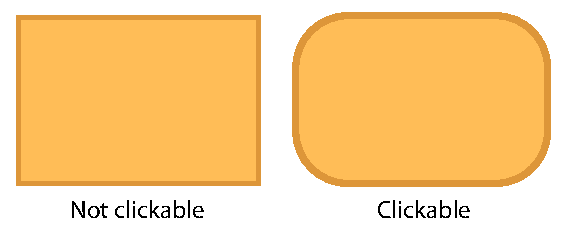
\includegraphics[scale=0.6]{gfx/buttons.pdf}
	\caption{Interactive element: Button illustration}
	\label{fig:buttons}
\end{figure}